\selectlanguage{italian}
\graphicspath{ {img/3/} }
\chapter{Neural Network e Convolutional Neural Network}\label{cap:NNeCNN}
\thispagestyle{empty} %Elimina il numero della prima pagina del capitolo.
\newpage

\section{\acf{NN}}
\vspace{8mm}


Ispirate dalla struttura del cervello, le \acf{NN} sono la risposta per rendere i computer capaci di compiere attività tipicamente svolte dall'uomo.
\subsection{Cosa sono le Neural Network?}

I cervelli umani interpretano il contesto delle situazioni del mondo reale in una maniera non concepibile dalle macchine. Le reti neurali furono sviluppate per la prima volta negli anni '50 per affrontare questo problema. Una rete neurale artificiale è un tentativo di simulare la rete di neuroni che formano un cervello umano in modo che il computer sia in grado di apprendere e prendere decisioni in modo umano. Le reti neurali vengono create programmando computer in maniera tale da comportarsi come se fossero cellule cerebrali interconnesse.
\subsection{Come funzionano le Neural Network?}

Le reti neurali artificiali utilizzano diversi livelli di elaborazione matematica per dare un senso alle informazioni che vengono fornite. Tipicamente, una rete neurale artificiale dispone di un numero variabile di neuroni artificiali, da dozzine a milioni di essi. I neuroni artificiali vengono chiamati unità, e sono disposti in una serie di strati. Il livello di input riceve varie forme di informazioni dal mondo esterno, tali informazioni sono i dati che la rete intende elaborare o conoscere. Dall'unità di input, i dati passano attraverso una o più unità nascoste. Il compito dell'unità nascosta è trasformare l'input in qualcosa che l'unità di output può usare.

La maggior parte delle reti neurali è completamente connessa da uno strato all'altro. Queste connessioni sono ponderate: maggiore è il numero, maggiore è l'influenza che un'unità ha su un'altra, simile a un cervello umano. Man mano che i dati passano attraverso ciascuna unità, la rete impara di più sui dati. Dall'altro lato della rete si trovano le unità di output: è qui che la rete risponde ai dati che sono stati forniti e processati.

Affinché le reti neurali possano apprendere, devono disporre di un'enorme quantità di informazioni che fanno parte del training set. Ad esempio, quando si cerca di insegnare ad una rete neurale come differenziare un gatto da un cane, il training set conterrà migliaia di immagini etichettate come immagini di cani e migliaia di immagini etichettate come immagini di gatti in modo da poter insegnare alla rete neurale tale differenza.


Una volta finita la fase di training, il modello prodotto proverà a classificare i dati futuri in base a ciò che viene percepito nelle diverse unità. Durante il periodo di addestramento, l'output della macchina viene confrontato con la descrizione fornita dall'uomo di ciò che dovrebbe essere osservato. Se sono uguali, la macchina è convalidata. Se non corrispondono, vengono utilizzate tecniche per regolare il suo apprendimento, andando indietro attraverso i livelli per modificare l'equazione matematica.
\newline
\begin{figure}[h!]
	\centering
	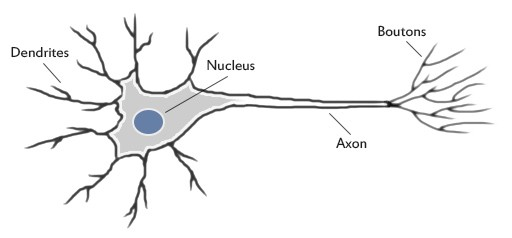
\includegraphics[width=100mm]{img/3/nn_1_1}
	\caption{\fontsize{10px}{0mm}\selectfont Biological Neuron \label{fig:nn_1_2}}
\end{figure}

\newpage
\subsection{Come modelliamo i neuroni artificiali?}

\begin{figure}[h!]
	\centering
	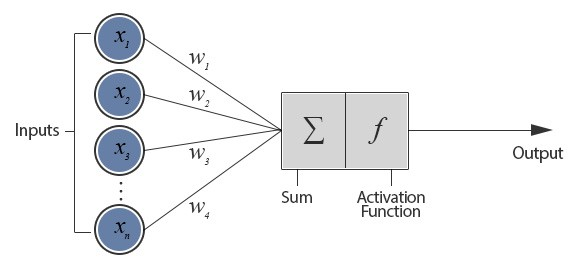
\includegraphics[width=100mm]{img/3/nn_1_2}
	\caption{\fontsize{10px}{0mm}\selectfont Artificial Neuron \label{fig:nn_1_2}}
\end{figure}



La figura rappresenta un neurone artificiale collegato con n altri neuroni artificiali che quindi riceve n input ($x_1$, $x_2$, ... $x_n$). Questa configurazione è chiamata \textbf{Perceptron}.
Gli ingressi ($x_1$, $x_2$,…. $x_n$) e i pesi ($w_1$, $w_2$,…. $w_n$) sono numeri reali che possono essere positivi o negativi.
Il Perceptron è costituito da pesi, da un processore di somma, da una funzione di attivazione e da un processore di soglia (noto come \textbf{bias}).
Il \textit{bias} di un algoritmo è l'insieme di assunzioni che il modello utilizza per prevedere gli output in base agli input non familiari, ossia non ancora incontrati, i pesi (\textit{weights}) invece sono delle costanti che indicano l'importanza della variabile associata nel determinare il valore dell'output del modello.

Tutti gli ingressi sono pesati individualmente, sommati e passati alla funzione di attivazione. Esistono molti tipi distinti di funzioni di attivazione, ma una delle più semplici è la funzione a gradini. Una funzione a gradini genererà output 1 se l'ingresso è superiore a una determinata soglia, altrimenti genererà output 0.
\newpage
Successivamente, verranno presentati i \textit{vettori di input} ottenuti da un training set, il Perceptron modificherà i pesi in base alla seguente equazione:


$$ \forall i \; W(i) = W(i) + A(T-A)*P(i) $$ 

Nota: in realtà l'equazione è 
$$W(i) = W(i) + a*g’*(T-A)*P(i)$$
dove $g’$ è la derivata della funzione di attivazione ed $a$ è il learning rate.
Il calcolo della derivata di una funzione a gradini può diventare complicato, inoltre esso non è di fondamentale importanza nella comprensione del topic in questione, quindi tale calcolo verrà ignorato.

$W$ è il vettore dei pesi, $P$ è il vettore di input, $T$ è l'output corretto che il Perceptron avrebbe dovuto conoscere e $A$ è l'ouput dato dal Perceptron stesso.

Quando tutti i vettori di training sono stati presentati al Perceptron e non si presentano errori, allora esso è stato allenato con successo.\newpage

\subsection{Cosa avviene nel Perceptron?}
Il perceptron, di volta in volta, somma tutti gli input e li separa in 2 categorie, quelli che causano un \emph{segnale di fire}\footnote{il nome deriva dalla biologia: quando i neuroni inviano un segnale nel cervello, si parla di firing} e quelli che non lo causano. Cioè, sta "disegnando" la linea:
$$w_1x_1 + w_2x_2 = t$$
I punti su un lato della linea rientrano in una categoria, i punti sull'altro lato rientrano nell'altra categoria.
La linea ottenuta è solo una delle infinite linee che possono essere ottenute per la separazione delle categorie.
\newline
\textbf{Limiti dei Perceptron}\newline
Non tutti gli insiemi di input possono essere divisi attraverso una linea. Nel caso in cui sia possibile, si parla di input \textit{linearmente separabili}. Se i vettori non sono linearmente separabili, la fase di apprendimento non raggiungerà mai un punto in cui tutti i vettori sono classificati in maniera corretta, e bisognerà utilizzare un approccio diverso.
\cite{MediumNN}
\newpage

\section{\acf{CNN}}
\vspace{8mm}
Le \acf{CNN} sono una categoria di reti neurali che si sono dimostrate molto efficaci in settori quali il riconoscimento e la classificazione delle immagini.
Le CNN, come le reti neurali (NN), sono costituite da neuroni con pesi e bias. Ogni neurone riceve diversi input, ne prende una somma, la passa attraverso una funzione di attivazione e risponde con un output, in pratica sembrano essere equivalenti alle reti neurali.
Diviene quindi naturale porsi la domanda: \textbf{Qual è la differenza tra CNN e NN?}\newline
Tra le varie differenze, la risposta è data dal fatto che le CNN hanno una caratteristica fondamentale: \textit{lavorano su volumi}, ossia, invece di ricevere in input un vettore di valori, ricevono in input un immagine, che è composta quindi da 3 vettori, uno per dimensione.

\newpage
\subsection{Convolution e funzionamento}

Per capire al meglio il funzionamento delle \acf{CNN} bisogna comprendere il concetto di \textbf{Convolution}(da cui il nome). Per farlo, utilizzeremo un filtro di dimensione arbitraria, in questo caso le dimensioni saranno 5x5x3.\newline
\begin{figure}[h!]
	\centering
	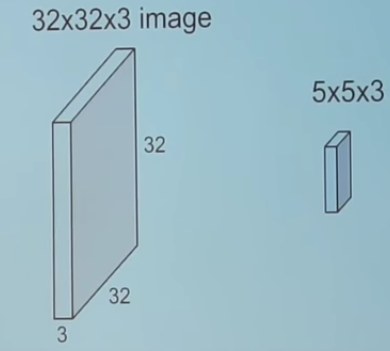
\includegraphics[width=80mm]{img/3/cnn_1_1}
	\caption{\fontsize{10px}{0mm}\selectfont Immagine e filtro considerati \label{fig:cnn_1_1}}
\end{figure}
\newpage
Una volta ottenuto il filtro, lo si fa scorrere sopra l'intera immagine e di volta in volta si calcola il prodotto tra il filtro e le sezioni dell'immagine sulle quali ci si trova, il risultato del prodotto sarà uno scalare.
\begin{figure}[h!]
	\centering
	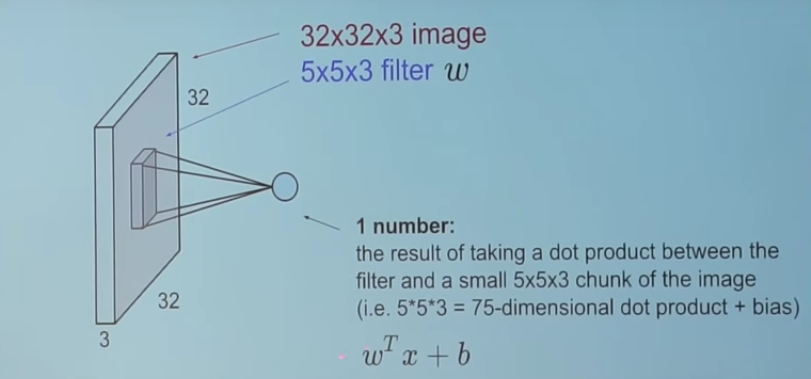
\includegraphics[width=110mm]{img/3/cnn_1_2}
	\caption{\fontsize{10px}{0mm}\selectfont Il prodotto appena descritto \label{fig:cnn_1_2}}
\end{figure}
\newline
Una volta calcolati tutti i prodotti si otterrà il seguente risultato:
\begin{figure}[h!]
	\centering
	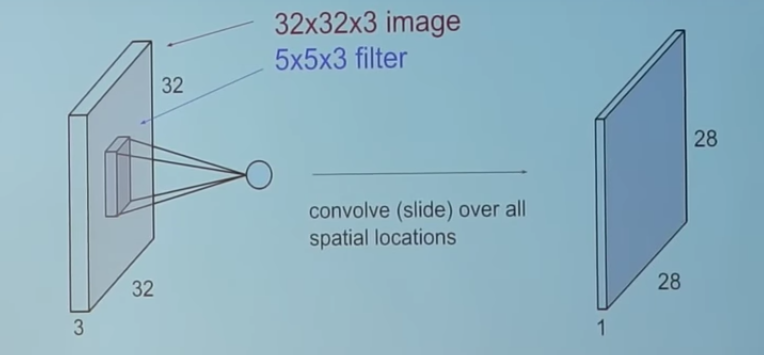
\includegraphics[width=110mm]{img/3/cnn_1_3}
	\caption{\fontsize{10px}{0mm}\selectfont Risultato finale \label{fig:cnn_1_3}}
\end{figure}
\newpage
Tornando alle CNN, si utilizza un cosiddetto \textbf{Convolutional Layer}(strato convoluzionale) che costituisce la parte fondamentale di una Convolutional Neural Network.
\begin{figure}[h!]
	\centering
	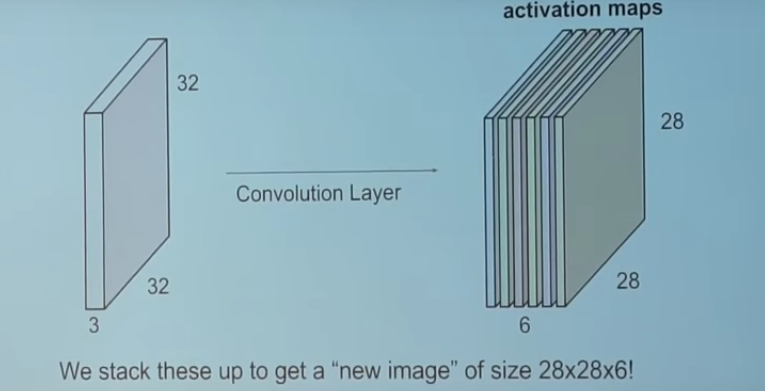
\includegraphics[width=110mm]{img/3/cnn_1_4}
	\caption{\fontsize{10px}{0mm}\selectfont Convolutional Layer \label{fig:cnn_1_4}}
\end{figure}
\newline
Lo strato convoluzionale contiene un insieme di filtri indipendenti(6 nell'esempio mostrato). Ogni filtro è convoluto con l'immagine indipendentemente dagli altri, risultando quindi in 6 \textit{feature maps} differenti(una feature map non è altro che l'output dell'applicazione del layer all'immagine).\cite{MediumCNN}

\subsection{Perchè non è stato utilizzato CNN?}\label{considerazioniCNN}
Come già detto precedentemente, le reti neurali convoluzionali sono una categoria di reti neurali molto efficaci per task di classificazione delle immagini. Nonostante ciò, durante l'attività di progettazione del software, in particolare durante la ricerca di Dataset contenenti immagini di iridi per il training della CNN, è stata riscontrata una notevole mancanza di dati: il dataset finale contiene 2500 immagini, da dividere in training set e test set, un numero piuttosto basso.
Tutto ciò, insieme alla estrema specificità dei dati causa overfitting da parte della CNN utilizzata, è stato quindi utilizzato un nuovo approccio: \emph{Viola-Jones} e \emph{Haar Cascades}
\newpage